\documentclass[10pt]{beamer}

\usepackage{lmodern}
\usepackage[utf8]{inputenc}
\usepackage[T1]{fontenc}		
\usepackage[english]{babel}

\usepackage{siunitx}

\usepackage{xcolor, colortbl}
\definecolor{darkgreen}{RGB}{0, 155, 85}

\definecolor{LOSS45}{RGB}{130,8,8}
\definecolor{LOSS3545}{RGB}{183,10,10}
\definecolor{LOSS2535}{RGB}{255,0,0}
\definecolor{LOSS1525}{RGB}{255,122,12}
\definecolor{LOSS0515}{RGB}{255,181,12}
\definecolor{STBL}{RGB}{215,215,215}
\definecolor{GAIN0515}{RGB}{58,255,12}
\definecolor{GAIN1525}{RGB}{58,178,12}
\definecolor{GAIN2535}{RGB}{56,136,17}
\definecolor{GAIN3545}{RGB}{50,119,16}
\definecolor{GAIN45}{RGB}{48,83,56}


\usepackage{graphicx}
\usepackage{floatrow}
\usepackage[
    scriptsize,
    labelformat=empty
]{caption}

\usepackage{enumitem}

\usepackage{standalone}

\usepackage{multirow}

\usepackage{array}
\newcolumntype{x}[1]{>{\centering\let\newline\\\arraybackslash\hspace{0pt}}m{#1}}
\usepackage{booktabs}
\usepackage{makecell}

\usepackage{tikz}
\usetikzlibrary{calc, 3d, shadows, decorations, shapes.arrows, fadings, trees, backgrounds}
\usepackage{pgfplots}
\usepackage{pgfplotstable}
\usepackage{forest}
\usepackage[final]{animate}

\usepackage{amsmath}
\usepackage{amsthm}
\usepackage{amsfonts}
\usepackage{amssymb}
\usepackage{mathrsfs}
\usepackage{bm}
\usepackage{bbold}
\usepackage{stmaryrd}
    
\usepackage[
    backend=biber,
    style=authoryear,
    dashed=false,
    sorting=nty,
    maxbibnames=5,
    minbibnames=5,
    maxcitenames=1,
    uniquelist=false,
    uniquename=false,
    hyperref=true,
    backref=true,
    backrefstyle=all+,
    isbn=false,
    url=false,
    doi=false
]{biblatex}
\usepackage{xpatch}

\addbibresource{references.bib}

\usepackage[acronym, toc, automake=true]{glossaries}

\usepackage{hyperref}
\hypersetup{
    % colorlinks=false,
    pdftitle={Semantic aware quality evaluation of 3D building models},
    pdfauthor={Oussama Ennafii},
    pdfkeywords={3D urban modeling} {buildings} {quality assessment} {taxonomy} {classification} {error detection} {geometry} {aerial imagery} {Very High Spatial Resolution} {Digital Surface Model},
    pdfstartview={FitH},
    unicode=true
}

\setbeamerfont{footnote}{size=\tiny}

\tikzset{
    invisible/.style={opacity=0},
    visible on/.style={alt=#1{}{invisible}},
    alt/.code args={<#1>#2#3}{
        \alt<#1>{\pgfkeysalso{#2}}{\pgfkeysalso{#3}}
    },
}    

\usepackage[useregional]{datetime2}

\usepackage{style/glossaries}

\usetheme{ign}

\title{Semantic aware quality evaluation of 3D building models}
\subtitle{A scalable approach}
\date{\tiny \DTMdisplaydate{2020}{1}{10}{5}}
\author{
    Oussama Ennafii
}

\begin{document}
    \begin{frame}[plain]
        \titlepage
    \end{frame}

    \section{Introduction}
        \subsection{Context}
            \begin{frame}{\texorpdfstring{\acrshort*{acr::3d}}{3D} building model}
                \begin{itemize}[label=\(\blacktriangleright\), font=\color{IGNGreen}]
                    \item<1-> \Acrfull{acr::3d} model \(\longleftrightarrow\) generalization of the building surface.
                    \item<only@2> Surface reconstruction \(\longleftrightarrow\) geometric fidelity;
                    \item<only@3> Generalization \(\longleftrightarrow\) reduce the complexity;
                    \item<only@4> Generalization \(\implies\) \textit{implicit} semantics;
                \end{itemize}
                \onslide<2->{
                    \begin{figure}[H]
                        \centering
                        \alt<2>{
                            \includestandalone[mode=buildnew, width=.8\textwidth]{figures/model_vs_mesh/mesh_model}
                            \caption{
                                \Gls{acr::3d} mesh of a building surface (\(\approx\) \num[output-exponent-marker = \text{e}]{1e5} triangles).
                            }
                        }{
                            \includestandalone[mode=buildnew, width=.8\textwidth]{figures/model_vs_mesh/ground_truth_model}
                            \caption{
                                Building \gls{acr::3d} (polyhedral) model (\(\approx\) \num{800} facets).
                            }
                        }
                    \end{figure}
                }
            \end{frame}

            \begin{frame}{\texorpdfstring{\acrfull*{acr::lod}}{Level of Detail}}
                \begin{figure}[H]
                    \centering
                    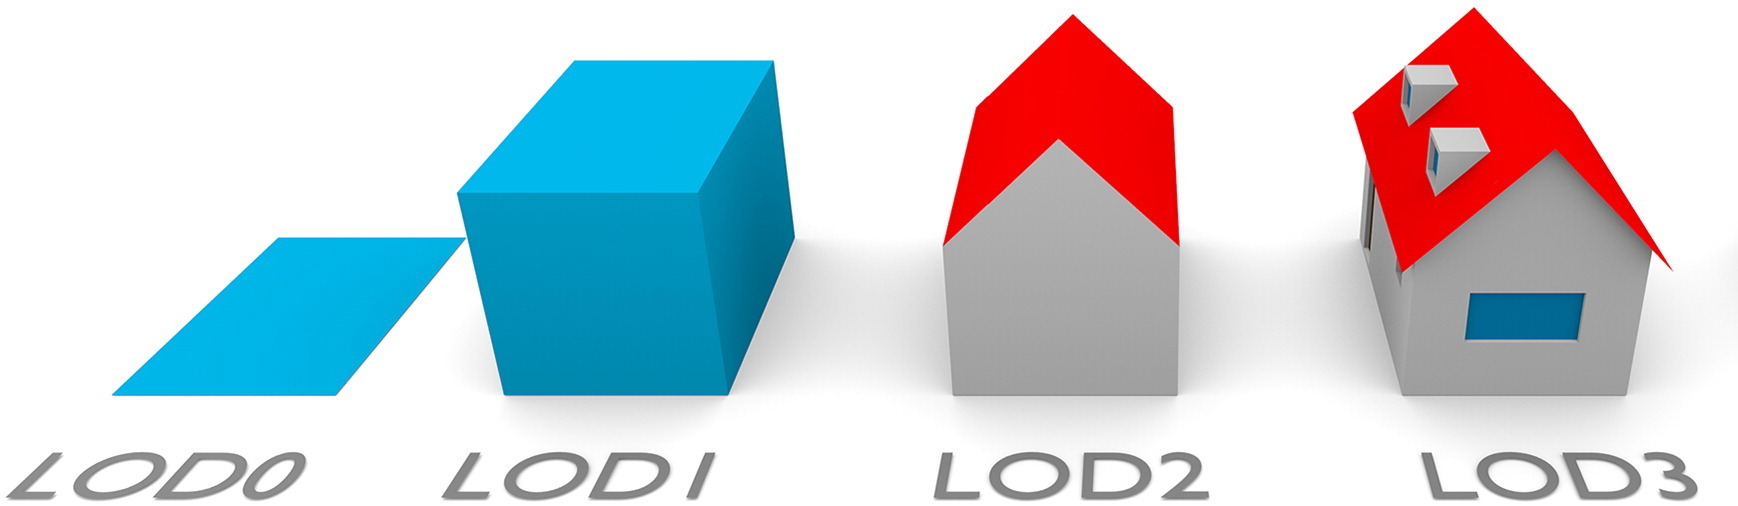
\includegraphics[width=\textwidth]{images/introduction/lods_3}
                    \caption{Considered \glspl{acr::lod} (Image taken from~\parencite{biljecki2016improved}).}
                \end{figure}
            \end{frame}

            \begin{frame}{Applications}
                \framesubtitle<1>{Physical simulation}
                \framesubtitle<2>{Planning}
                \framesubtitle<3>{Entertainement}

                \temporal<2>{
                    \begin{figure}[H]
                        \centering
                        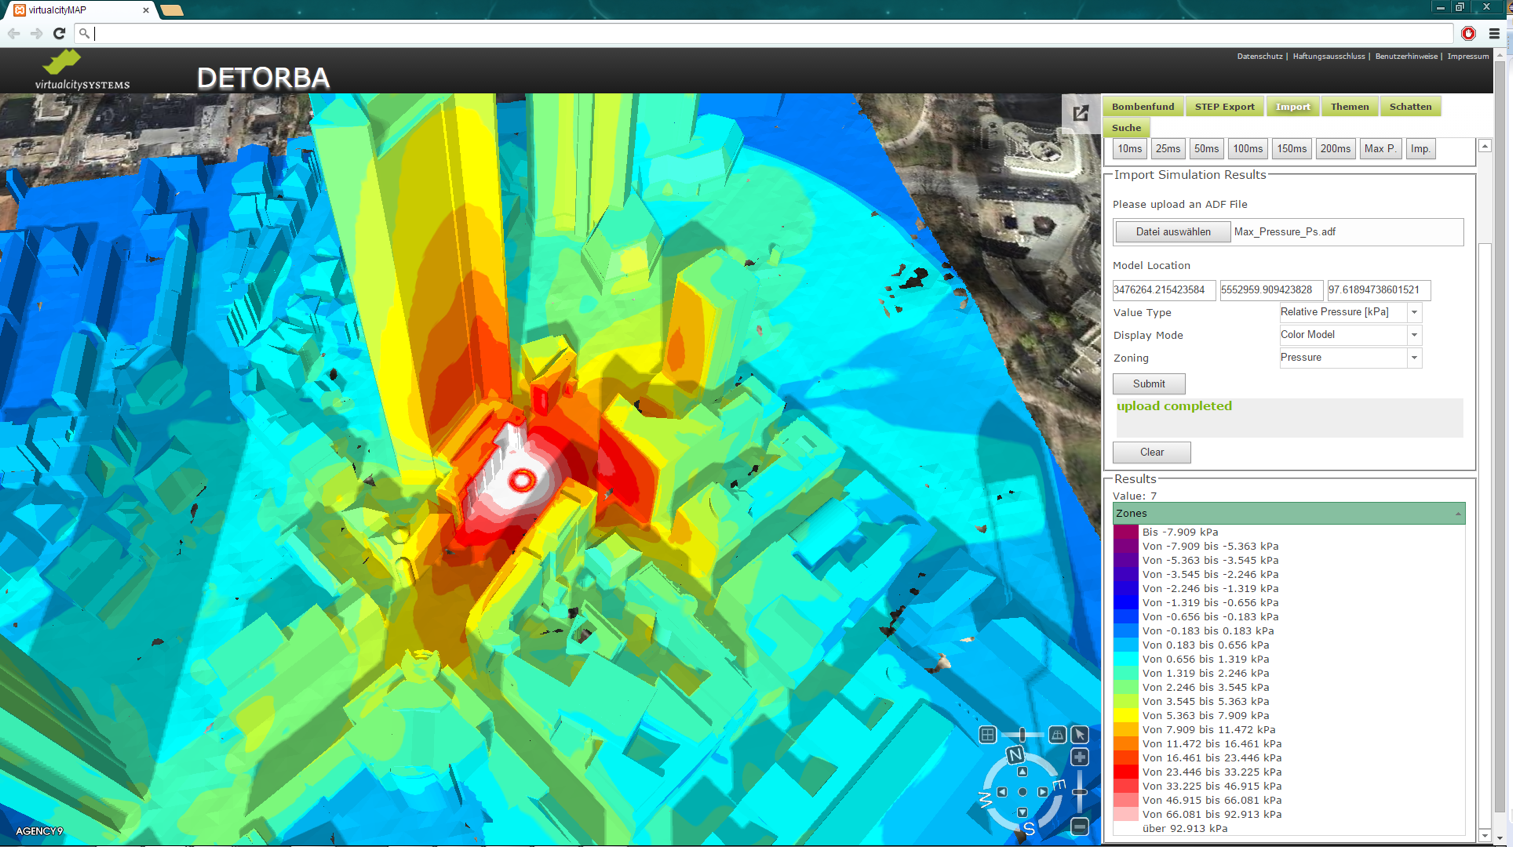
\includegraphics[width=.8\textwidth]{images/introduction/3d_model_applications/explosion_simulation}
                        \caption{Explosion simulation (Image taken from~\parencite{biljecki2015applications}).}
                    \end{figure}
                }
                {
                    \begin{figure}[H]
                        \centering
                        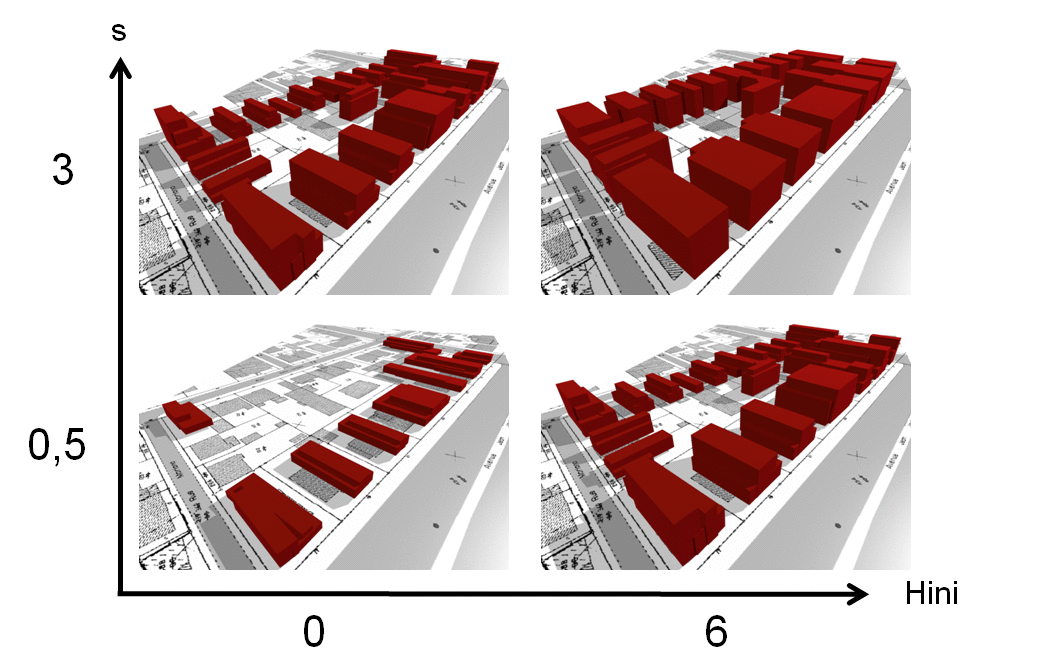
\includegraphics[width=.8\textwidth]{images/introduction/3d_model_applications/simplu}
                        \caption{Example of \gls{acr::3d} urban scene simulated based on known urban norms (Image taken from~\parencite{brasebin2017stochastic}).}
                    \end{figure}
                }
                {
                    \begin{figure}[H]
                        \centering
                        \animategraphics[autoplay, loop, width=.8\textwidth]{20}{images/introduction/3d_model_applications/trocadero/trocadero-}{0}{73}
                        \caption{Mixed reality for historical applications using iTowns\footnotemark platform (Credits to A. Devaux\footnotemark).}
                    \end{figure}
                    \footnotetext{
                        \href{http://www.itowns-project.org}{iTowns project.}
                    }
                    \addtocounter{footnote}{1}
                    \footnotetext{
                        \href{http://recherche.ign.fr/labos/matis/~devaux}{Alexandre Devaux website.}
                    }
                }
            \end{frame}

            \begin{frame}{\texorpdfstring{\acrshort*{acr::3d}}{3D} building modeling}
                \centering
                \includestandalone[mode=buildnew, width=\textwidth]{figures/context}
            \end{frame}

        \subsection{Motivation}
            \begin{frame}{Modeling errors}{Different point of views}
                \begin{itemize}[label=\(\blacktriangleright\), font=\color{IGNGreen}]
                    \item<1-> Errors in format: compliant to CityGML\footfullcite{ledoux2013validation} \dots.
                    \item<2-> Errors in fidelity (geometry)\uncover<2->{\footfullcite{berger2013benchmark}}.
                    \item<3-> Errors in generalization.
                \end{itemize}
            \end{frame}

            \begin{frame}{Need for semantics}
                \begin{itemize}[label=\(\blacktriangleright\), font=\color{IGNGreen}]
                    \item<1-> Modeling \(\longleftrightarrow\) compromise between:
                    \begin{itemize}[label=\(\blacktriangleright\), font=\color{IGNGreen}]
                        \item<2-> geometric accuracy;
                        \item<3-> and \textit{implicit} semantics.
                    \end{itemize}
                    \item<4-> Errors are \underline{geometric} and \underline{semantic} in nature.
                \end{itemize}
            \end{frame}
        
            \begin{frame}{Goal}
                \begin{itemize}[label=\(\blacktriangleright\), font=\color{IGNGreen}]
                    \item<1-> \underline{Define errors} that affects building \gls{acr::3d} models.
                    \item<2-> Devise a method for \underline{error detection}.
                \end{itemize}
            \end{frame}

            \begin{frame}{Challenges}
                \begin{itemize}[label=\(\blacktriangleright\), font=\color{IGNGreen}]
                    \item<1-> \underline{Scalability} up to city level;
                    \item<2-> Genericity towards:
                        \begin{itemize}
                            \item<3-> modeling approach;
                            \item<4-> urban scene.
                        \end{itemize}
                    \item<5-> Automation with the least human intervention possible.
                \end{itemize}
            \end{frame}

        \begin{frame}{State of the art}
            \centering
            \includestandalone[mode=buildnew, width=\textwidth]{figures/state_of_the_art}
        \end{frame}

        \begin{frame}{Contributions}
            \begin{itemize}[label=\(\blacktriangleright\), font=\color{IGNGreen}, itemsep=2em]
                \item<1-> Semantic error taxonomy;
                \item<2-> Learning evaluation approach;
                \item<3-> Experimental validation.
            \end{itemize}
        \end{frame}

    \section{Semantic evaluation}
        \subsection{Design principles}
            \begin{frame}{Hierarchization and Modularity}
                \begin{itemize}[label=\(\blacktriangleright\), font=\color{IGNGreen}, itemsep=2em]
                    \item<1-> Hierarchization:
                        \begin{itemize}[label=\(\blacktriangleright\), font=\color{IGNGreen}, itemsep=2em]
                            \item<2-> \underline{Iteratively} define more and more specific errors;
                            \item<3-> Each \underline{specificity level}: the most possible \texttt{Generability}.
                        \end{itemize}
                    \item<4-> Modularity:
                        \begin{itemize}[label=\(\blacktriangleright\), font=\color{IGNGreen}, itemsep=2em]
                            \item<5-> An error \(\equiv\) Composition of \underline{basic errors} common to all scenes.
                        \end{itemize}
                \end{itemize}
            \end{frame}
        
        \subsection{General layout}
            \begin{frame}{Error classification}
                \includestandalone[mode=buildnew, width=\textwidth]{figures/taxonomy_tree_animated}
            \end{frame}

            \begin{frame}{\texttt{Atomic errors}}
                \begin{itemize}[label=\(\blacktriangleright\), font=\color{IGNGreen}]
                    \item<1-> \Acrfull{acr::2d} errors:
                        \begin{itemize}[label=\(\blacktriangleright\), font=\color{IGNGreen}]
                            \item<only@2-10> Segmentation issue (semantic):
                                \begin{itemize}
                                    \item<only@3-6> Under segmentation;
                                    \item<only@7-10> Over segmentation.      
                                \end{itemize}
                            \item<only@11-19> Border issue (geometric):
                            \begin{itemize}
                                \item<only@12-15> Inaccurate topology;
                                \item<only@16-19> Imprecise border.      
                            \end{itemize}
                        \end{itemize}
                    \item<only@20-> \gls{acr::3d} error (geometric):
                        \begin{itemize}[label=\(\blacktriangleright\), font=\color{IGNGreen}]
                            \item<only@21-> Imprecise geometry.
                        \end{itemize}
                \end{itemize}
                \begin{overlayarea}{\textwidth}{.5\textheight}
                    \only<3-6>{
                        \begin{figure}[H]
                            \centering
                            \alt<3-4>{
                                \alt<3>{
                                \includestandalone[mode=buildnew, height=.4\textheight]{figures/errors/building/bos}
                                \includestandalone[mode=buildnew, height=.4\textheight]{figures/errors/building/bus}
                                }{
                                    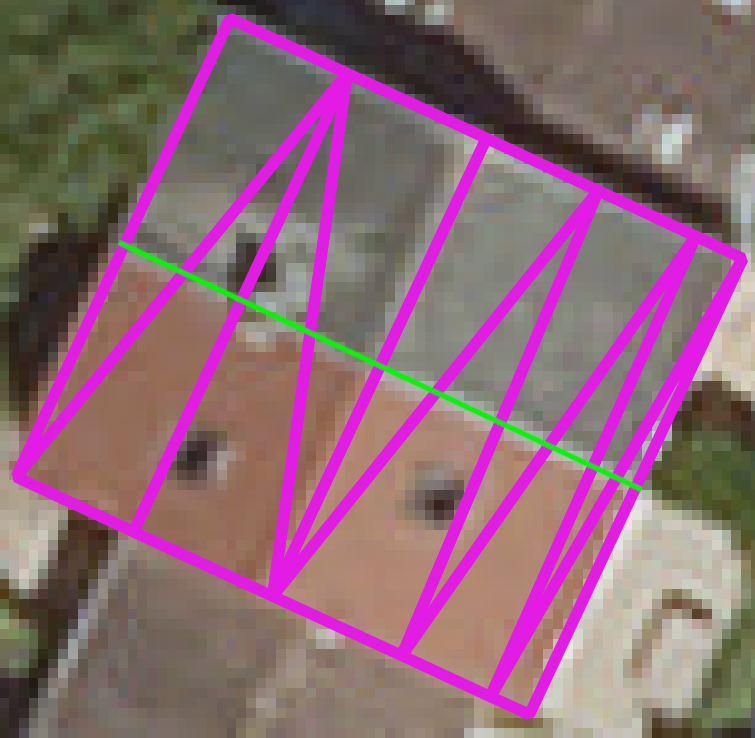
\includegraphics[height=.4\textheight]{images/errors/building/under_segmentation}
                                }
                            }{
                                \alt<5>{
                                    \includestandalone[mode=buildnew, height=.4\textheight]{figures/errors/facet/correct_fos_fus_fib_fig}
                                    \includestandalone[mode=buildnew, height=.4\textheight]{figures/errors/facet/fus}
                                }{
                                    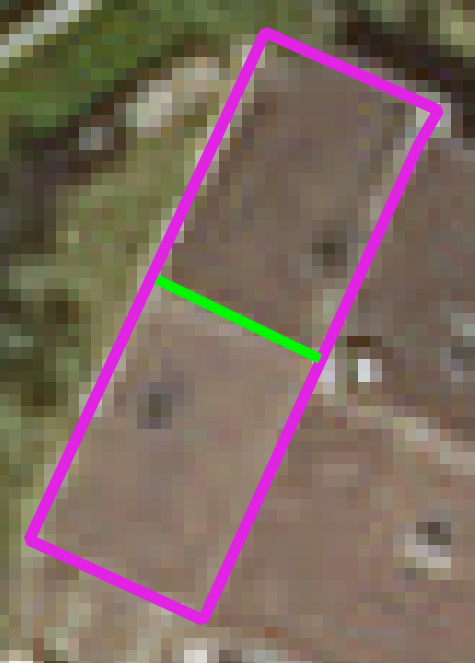
\includegraphics[height=.4\textheight, angle=270]{images/errors/facet/under_segmentation}
                                }
                            }
                            \caption{
                                \alt<3-4>{
                                    \alt<3>{
                                        Ground truth buildings are in different colors: \textcolor{cyan}{blue} and \textcolor{green}{green}.
                                    }{
                                        Nadir projection of an erroneous building superposed on the corresponding orthoimage.
                                    }
                                }{
                                    \alt<5>{
                                        \textcolor{cyan}{Blue} \(\leftrightarrow\) under-segmented facet.
                                    }{
                                        Nadir projection: \textcolor{red}{red} \(\leftrightarrow\) inexisting edges.
                                    }
                                }
                            }
                        \end{figure}
                    }
                    \only<7-10>{
                        \begin{figure}[H]
                            \centering
                            \alt<7-8>{
                                \alt<7>{
                                    \includestandalone[mode=buildnew, height=.4\textheight]{figures/errors/building/bus}
                                    \includestandalone[mode=buildnew, height=.4\textheight]{figures/errors/building/bos}
                                }{
                                    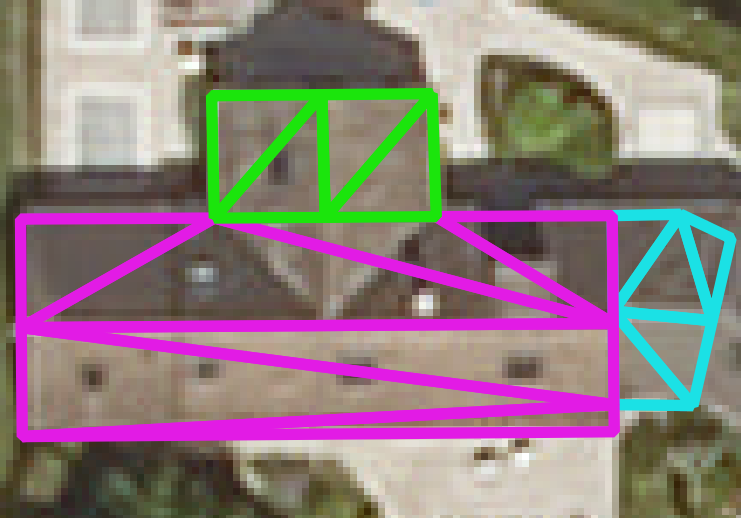
\includegraphics[height=.4\textheight]{images/errors/building/over_segmentation}
                                }
                            }{
                                \alt<9>{
                                    \includestandalone[mode=buildnew, height=.4\textheight]{figures/errors/facet/correct_fos_fus_fib_fig}
                                    \includestandalone[mode=buildnew, height=.4\textheight]{figures/errors/facet/fos}
                                }{
                                    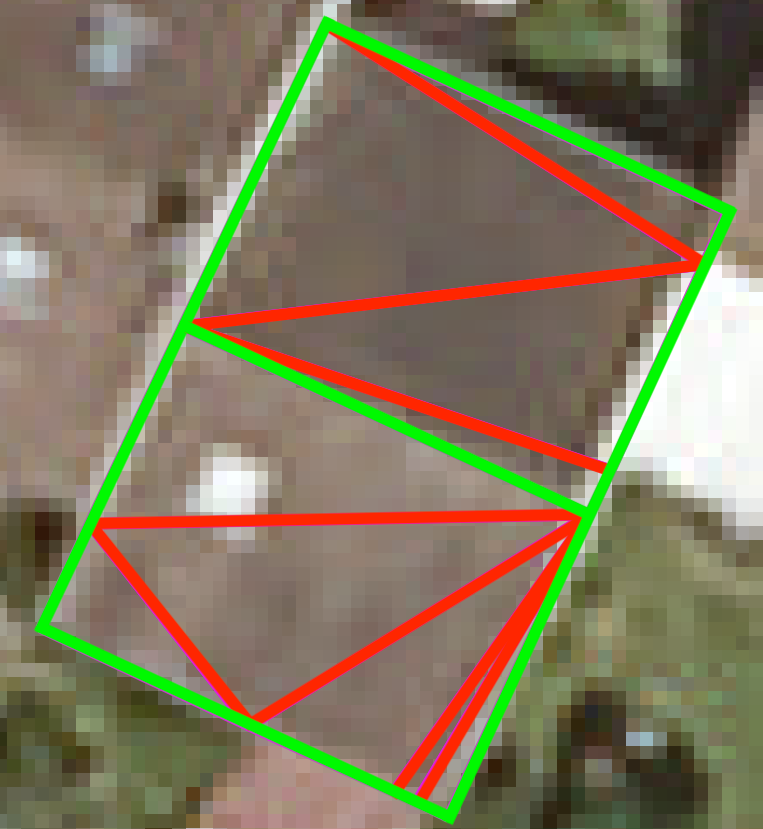
\includegraphics[height=.4\textheight]{images/errors/facet/over_segmentation}
                                }
                            }
                            \caption{
                                \alt<7-8>{
                                    \alt<7>{
                                        Modeled buildings are in different colors: \textcolor{cyan}{blue} and \textcolor{green}{green}.
                                    }{
                                        Nadir projection: \textcolor{green}{green} \(\leftrightarrow\) unmodeled edge.
                                    }
                                }{
                                    \alt<9>{
                                        \textcolor{green}{Green} \(\leftrightarrow\) inexisting edges.
                                    }{
                                        Nadir projection of an erroneous building superposed on the corresponding orthoimage.
                                    }
                                }
                            }
                        \end{figure}
                    }
                    \only<12-15>{
                        \begin{figure}[H]
                            \centering
                            \alt<12-13>{
                                \alt<12>{
                                    \includestandalone[mode=buildnew, height=.4\textheight]{figures/errors/building/correct_bit}
                                    \includestandalone[mode=buildnew, height=.4\textheight]{figures/errors/building/bit}
                                }{
                                    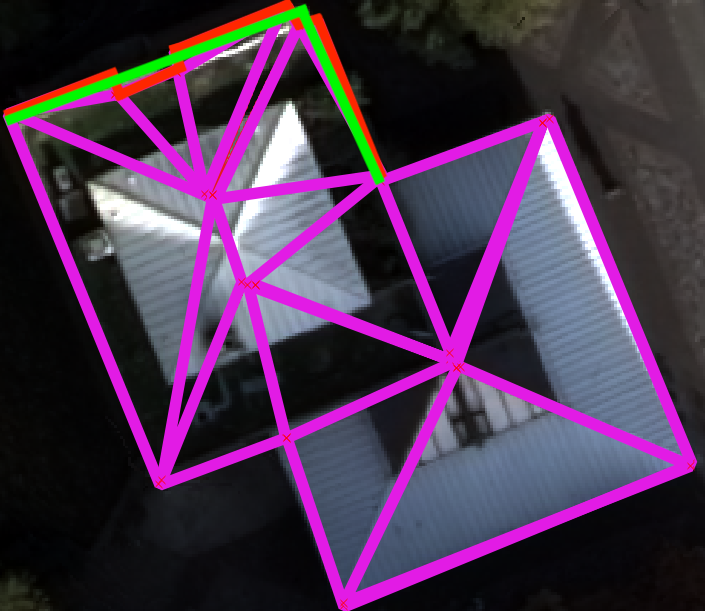
\includegraphics[height=.4\textheight]{images/errors/building/topology}
                                }
                            }{
                                \alt<14>{
                                    \includestandalone[mode=buildnew, height=.4\textheight]{figures/errors/facet/correct_fit}
                                    \includestandalone[mode=buildnew, height=.4\textheight]{figures/errors/facet/fit}
                                }{
                                    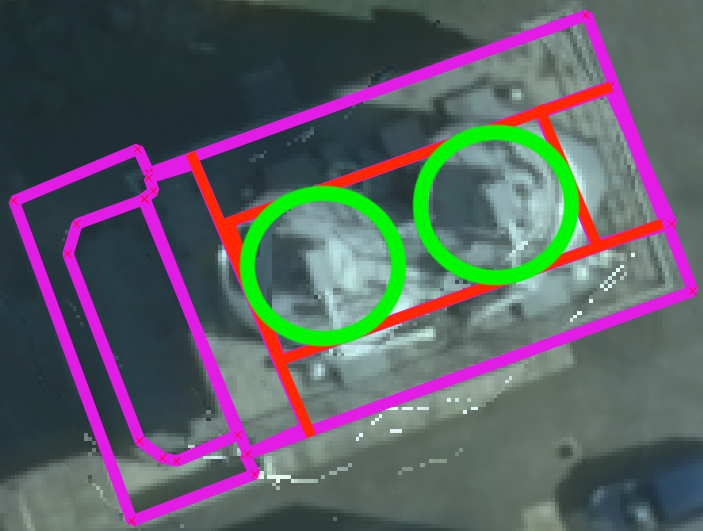
\includegraphics[height=.4\textheight]{images/errors/facet/topology}
                                }
                            }
                            \caption{
                                \alt<12-13>{
                                    \alt<12>{
                                        \textcolor{olive}{Yellow} \(\leftrightarrow\) inaccurate borders.
                                    }{
                                        Nadir projection: \textcolor{green}{green} \(\leftrightarrow\) ground truth and \textcolor{red}{red} \(\leftrightarrow\) the model.
                                    }
                                }{
                                    \alt<14>{
                                        \textcolor{olive}{Yellow} \(\leftrightarrow\) inaccurate borders.
                                    }{
                                        Nadir projection: \textcolor{green}{green} \(\leftrightarrow\) ground truth and \textcolor{red}{red} \(\leftrightarrow\) the model.
                                    }
                                }
                            }
                        \end{figure}
                    }
                    \only<16-19>{
                        \begin{figure}[H]
                            \centering
                            \alt<16-17>{
                                \alt<16>{
                                    \includestandalone[mode=buildnew, height=.4\textheight]{figures/errors/building/correct_bib}
                                    \includestandalone[mode=buildnew, height=.4\textheight]{figures/errors/building/bib}
                                }{
                                    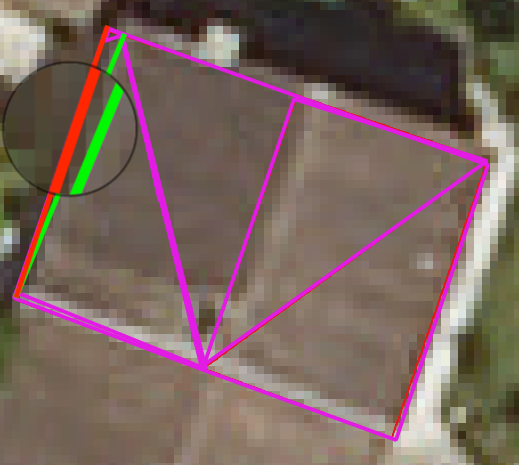
\includegraphics[height=.4\textheight]{images/errors/building/border}
                                }
                            }{
                                \alt<18>{
                                    \includestandalone[mode=buildnew, height=.4\textheight]{figures/errors/facet/correct_fos_fus_fib_fig}
                                    \includestandalone[mode=buildnew, height=.4\textheight]{figures/errors/facet/fib}
                                }{
                                    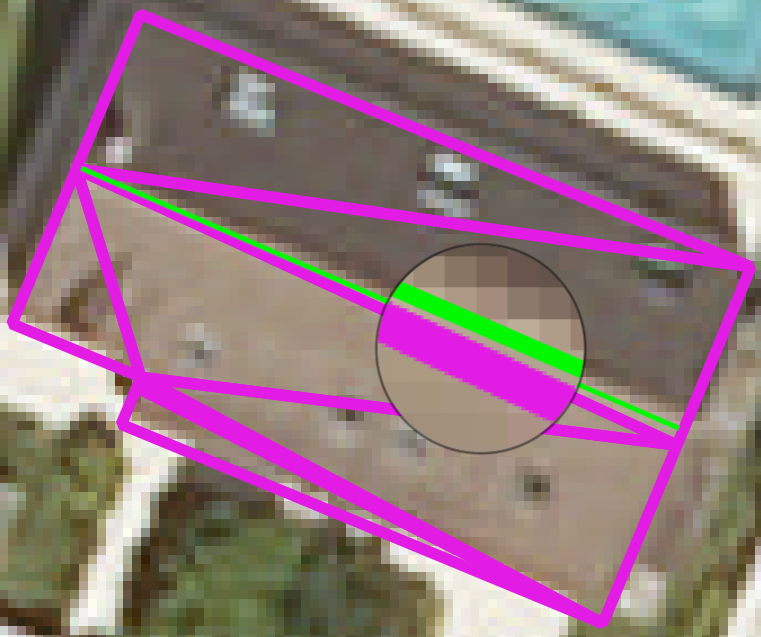
\includegraphics[height=.4\textheight]{images/errors/facet/border}
                                }
                            }
                            \caption{
                                \alt<16-17>{
                                    \alt<16>{
                                        \textcolor{red}{Red} \(\leftrightarrow\) imprecise borders.
                                    }{
                                        Nadir projection: \textcolor{green}{green} \(\leftrightarrow\) ground truth and \textcolor{red}{red} \(\leftrightarrow\) the model.
                                    }
                                }{
                                    \alt<18>{
                                        \textcolor{red}{Red} \(\leftrightarrow\) imprecise borders.
                                    }{
                                        Nadir projection: \textcolor{green}{green} \(\leftrightarrow\) ground truth.
                                    }
                                }
                            }
                        \end{figure}
                    }
                    \only<21-23>{
                        \begin{figure}[H]
                            \centering
                            \alt<21>{
                                \includestandalone[mode=buildnew, height=.4\textheight]{figures/errors/building/correct_big}
                                \includestandalone[mode=buildnew, height=.4\textheight]{figures/errors/building/big}
                            }{
                                \alt<22>{
                                    \includestandalone[mode=buildnew, height=.4\textheight]{figures/errors/facet/correct_fos_fus_fib_fig}
                                    \includestandalone[mode=buildnew, height=.4\textheight]{figures/errors/facet/fig}
                                }{
                                    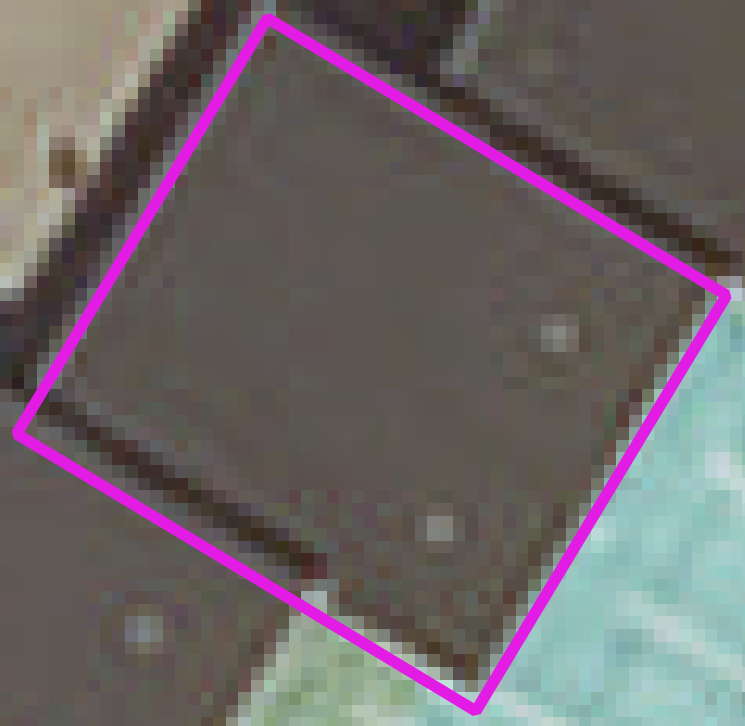
\includegraphics[height=.4\textheight]{images/errors/facet/geometry}
                                }
                            }
                            \caption{
                                \alt<21>{
                                    \textcolor{violet}{Purple} \(\leftrightarrow\) imprecise facet.
                                }{
                                    \alt<22>{
                                        \textcolor{violet}{Purple} \(\leftrightarrow\) imprecise facet.
                                    }{
                                        Nadir projection: slanted facet (\SI{25}{\degree}) modeled as horizontal.
                                    }
                                }
                            }
                        \end{figure}
                    }
                \end{overlayarea}
            \end{frame}

    \section{Learned evaluation}
        \begin{frame}{Evaluation is classification}
            \begin{itemize}[label=$\blacktriangleright$, font=\color{IGNGreen}]
                \item<1-> Evaluation at \underline{building level};
                \item<2-> Error detection \(\leftrightarrow\) supervized classification;
                \item<3-> Respects both constraints:
                    \begin{itemize}[label=$\blacktriangleright$, font=\color{IGNGreen}]
                        \item<4-> \textbf{Large-scale}: prediction on unseen instances;
                        \item<5-> \textbf{Automation}: needs manual annotations.
                    \end{itemize}
            \end{itemize}
        \end{frame}

        \begin{frame}{The evaluation pipeline}
            \begin{figure}[H]
                \includestandalone[mode=buildnew, height=.75\textheight]{figures/graphical_pipeline}
            \end{figure}
        \end{frame}

        \subsection{Baseline}
            \begin{frame}{Geometric features}
                \centering
                \includestandalone[mode=buildnew, width=.75\textwidth]{figures/features/geometric_animated}
            \end{frame}
            \begin{frame}{Height based features}
                \centering
                \includestandalone[mode=buildnew, width=\textwidth]{figures/features/height_based_animated}                
            \end{frame}
            \begin{frame}{Image based features}
                \centering
                \includestandalone[mode=buildnew, width=.8\textwidth]{figures/features/image_based_animated}                
            \end{frame}
    \section{Experiments}
        \begin{frame}{Datasets: urban scenes}
            \centering
            \includestandalone[mode=buildnew, width=.9\textwidth]{figures/dataset}
        \end{frame}
        \begin{frame}{Ablation study: Elancourt example}
            \begin{table}[H]
                \scriptsize
                \begin{center}
                    \scriptsize
                    \begin{tabular}{|x{.5cm} | x{.8cm} x{.8cm} | x{.9cm} x{.9cm} | x{.8cm} x{.8cm} | x{.8cm} x{.8cm}|}
                        \hline
                        &\multicolumn{2}{x{1.6cm}|}{\textbf{Geom.}} & \multicolumn{2}{x{1.8cm}|}{\textbf{Geom. $\cup$ Hei.}} & \multicolumn{2}{x{1.6cm}|}{\textbf{Geom. $\cup$ Im.}} & \multicolumn{2}{x{1.6cm}|}{\textbf{All}}\\
                        \cline{2-9}
                        &\textbf{Rec.} & \textbf{Prec.} & \textbf{Rec.} & \textbf{Prec.} & \textbf{Rec.} & \textbf{Prec.} & \textbf{Rec.} & \textbf{Prec.}\\
                        \hline
                        \texttt{BOS} & \textbf{93.96} & 76.15 & 91.43 & \textbf{77.76} & 91.51 & 76.08 & 90.83 & 76.14 \\
                        \hline
                        \strut\\[-\normalbaselineskip]
                        \only<3|handout:0>{\\[-\normalbaselineskip]\rowcolor{IGNGreen}}\texttt{BUS} & 32.98 & \textbf{76.47} & \textbf{41.86} & 75.57 & 40.38 & 71.00 & 39.32 & 71.81 \\
                        \hline
                        \strut\\[-\normalbaselineskip]
                        \only<5|handout:0>{\\[-\normalbaselineskip]\rowcolor{IGNRed}}\texttt{BIB} & 12.32 & 67.57 & 12.81 & \textbf{68.42} & 16.26 & 67.35 & \textbf{16.75} & 68.0 \\
                        \hline
                        \strut\\[-\normalbaselineskip]
                        \only<4|handout:0>{\\[-\normalbaselineskip]\rowcolor{orange}}\only<5|handout:0>{\\[-\normalbaselineskip]\rowcolor{IGNRed}}\texttt{BIT} & \textbf{25.25} & 92.59 & 20.20 & 90.91 & 20.20 & \textbf{95.24} & 11.11 & 91.67 \\
                        \hline
                        \hline
                        \texttt{FOS} & 98.91 & 99.07 & 98.91 & \textbf{99.30} & \textbf{98.99} & 98.84 & 98.91 & 98.84 \\
                        \hline
                        \strut\\[-\normalbaselineskip]
                        \only<5|handout:0>{\\[-\normalbaselineskip]\rowcolor{IGNRed}}\texttt{FUS} & \textbf{1.90} & 54.55 & 0.63 & \textbf{66.67} & 1.61 & 50 & 1.27 & \textbf{66.67} \\
                        \hline
                        \strut\\[-\normalbaselineskip]
                        \only<5|handout:0>{\\[-\normalbaselineskip]\rowcolor{IGNRed}}\texttt{FIB} & \textbf{9.17} & 87.5 & 0 & --- & 8.30 & 82.61 & 7.42 & \textbf{100} \\
                        \hline
                        \strut\\[-\normalbaselineskip]
                        \only<5|handout:0>{\\[-\normalbaselineskip]\rowcolor{IGNRed}}\texttt{FIT} & \textbf{6.67} & \textbf{100} & 8.73 & 95.24 & 3.33 & \textbf{100} & 3.33 & \textbf{100} \\
                        \hline
                        \texttt{FIG} & \textbf{80.54} & 73.14 & 80.45 & \textbf{72.62} & 78.69 & 72.12 & 79.02 & 71.82 \\
                        \hline
                    \end{tabular}
                \end{center}
            \end{table}
            % \only<1>{
            %     \begin{center}
            %         \footnotesize Results in percentage obtained using \texttt{RF} (\underline{1,000 trees} \& \underline{max depth 4}) and \underline{10-fold cross. val}.
            %     \end{center}
            % }
            \begin{itemize}[label=\(\blacktriangleright\), font=\color{IGNGreen}]
                \item[\textcolor{IGNDarkGreen}{\(\blacktriangleright\)}]<2-> \footnotesize In most cases \textbf{Geom.} is sufficient;
                \item<3-> \footnotesize Except for \texttt{BUS} $\rightarrow$ other modalities have a big impact ($\approx$ + 10\%).
                \item[\textcolor{orange}{\(\blacktriangleright\)}]<4-> \footnotesize Only \textbf{Geom.} is even \underline{the best} for \texttt{BIT}.
                \item[\textcolor{IGNRed}{\(\blacktriangleright\)}]<5-> \footnotesize Highly unbalanced labels are \underline{hard} to detect.
            \end{itemize}
        \end{frame}
        \begin{frame}{Transferability}
            \begin{table}[H]
                \scriptsize
                \begin{center}
                    \begin{tabular}{| x{1.5cm}| x{.4cm} | x{.4cm} | x{.4cm} | x{.4cm} | x{.4cm} | x{.4cm} | x{.4cm} | x{.4cm} | x{.4cm} |}
                        \hline
                        &\texttt{BOS}  & \texttt{BUS} &\texttt{BIB} &\texttt{BIT} &\texttt{FOS}  & \texttt{FUS} &\texttt{FIB} &\texttt{FIT} &\texttt{FIG} \\
                        \hline
                        Elancourt $\rightarrow$ Nantes &\cellcolor{IGNRed} & \cellcolor{IGNRed}&\cellcolor{IGNRed}& \cellcolor{IGNRed}& \cellcolor{IGNGreen}& \cellcolor{IGNGreen}&\cellcolor{IGNGreen} Im. & \cellcolor{IGNRed}&\cellcolor{IGNGreen}\\
                        \hline
                        Elancourt $\rightarrow$ Paris-13  & \cellcolor{IGNRed}& \cellcolor{IGNRed}& \cellcolor{IGNGreen}& \cellcolor{IGNRed}& \cellcolor{IGNGreen}& \cellcolor{IGNGreen}Im.& \cellcolor{IGNGreen}Im.& \cellcolor{IGNRed}&\cellcolor{IGNGreen}\\
                        \hline
                        Nantes $\rightarrow$ Paris-13  & \cellcolor{IGNRed}& \cellcolor{IGNRed}& \cellcolor{IGNDarkGrey} & \cellcolor{IGNGreen}& \cellcolor{IGNGreen}& \cellcolor{IGNGreen}& \cellcolor{IGNGreen}& \cellcolor{IGNDarkGrey} &\cellcolor{IGNGreen}\\
                        \hline
                        Nantes $\rightarrow$ Elancourt  &\cellcolor{IGNGreen} & \cellcolor{IGNRed}& \cellcolor{IGNRed}&\cellcolor{IGNGreen}All & \cellcolor{IGNGreen}& \cellcolor{IGNRed}&\cellcolor{IGNRed}Im. &\cellcolor{IGNGreen}Im. &\cellcolor{IGNGreen}\\
                        \hline
                        Paris-13 $\rightarrow$ Nantes  &\cellcolor{IGNRed} & \cellcolor{IGNRed}& \cellcolor{IGNDarkGrey} & \cellcolor{IGNGreen}&\cellcolor{IGNGreen} & \cellcolor{IGNRed}& \cellcolor{IGNGreen}& \cellcolor{IGNDarkGrey} & \cellcolor{IGNRed} Hei.\\
                        \hline
                        Paris-13 $\rightarrow$ Elancourt &\cellcolor{IGNGreen} &\cellcolor{IGNRed} & \cellcolor{IGNGreen}Im. & \cellcolor{IGNGreen}& \cellcolor{IGNGreen}& \cellcolor{IGNRed}& \cellcolor{IGNRed}Im. & \cellcolor{IGNDarkGrey} & \cellcolor{IGNGreen}\\
                        \hline
                    \end{tabular}
                    \caption{\footnotesize \textcolor{IGNRed}{$\blacksquare$}: Loss in F-score, \textcolor{IGNGreen}{$\blacksquare$}: Stability or gain in F-score.}
                \end{center}
            \end{table}
            \uncover<2->{
                \begin{itemize}[label=\(\blacktriangleright\), font=\color{IGNGreen}]
                    \item<2-> \footnotesize Only 8/24 of \texttt{Building errors} transferability cases are \textcolor{IGNGreen}{positive}.
                    \item<3-> \footnotesize \texttt{Facets errors} are more transferable: 19/30 are \textcolor{IGNGreen}{positive}.
                    \item<4-> \footnotesize Additional modalities play a \underline{critical role} in error prediction.
                \end{itemize}
            }
        \end{frame}
        
    \section{Conclusion}
        \begin{frame}{\textcolor{yellow}{Conclusion} \& \textcolor{purple}{Perspectives}}
            \begin{itemize}[label=\(\blacktriangleright\), font=\color{yellow}, itemsep=2em]
                \item<1-> \textbf{Hierarchical and modular} taxonomy;
                \item<2-> \textbf{Fast, lightweight and modular} pipeline for model evaluation;
                \item<3-> Pipeline tested with \textbf{baseline} and \textbf{advanced} handcrafted features:
                    \begin{itemize}[label=\(\blacktriangleright\), font=\color{IGNGreen}]
                        \item<4-> Geometric features are often sufficient for error prediction;
                        \item<5-> Adding modalities is most helpfull for transferability.
                    \end{itemize}
            \end{itemize}
            \uncover<6->{
                ~\\
                Future work:
                \begin{itemize}[label=\(\blacktriangleright\), font=\color{purple}, itemsep=2em]
                    \item<6-> Use of deep learning.
                    \item<7-> Dataset augmentation $\longrightarrow$ \textbf{Simulate errors}.
                \end{itemize}
            }
        \end{frame}
\end{document}
